\documentclass{article} 
\usepackage{iclr2026_conference,times}

% Optional math commands from https://github.com/goodfeli/dlbook_notation.
\input{math_commands.tex}

\usepackage{hyperref}
\usepackage{url}
\usepackage{booktabs}
\usepackage{graphicx}

\title{Reproducing the Clipping Stability Claim in\\Proximal Policy Optimization}

% Authors must not appear in the submitted version. They should be hidden
% as long as the \iclrfinalcopy macro remains commented out below.
% Non-anonymous submissions will be rejected without review.
\author{Anonymous}

\newcommand{\fix}{\marginpar{FIX}}
\newcommand{\new}{\marginpar{NEW}}

%\iclrfinalcopy % Uncomment for camera-ready version, but NOT for submission.
\begin{document}

\maketitle

\begin{abstract}
This project reproduces the stability claim of \citep{schulman2017ppo}: that the clipped surrogate objective ($L^{CLIP}$) from Proximal Policy Optimization (PPO) produces more stable training dynamics than the unclipped surrogate ($L^{CPI}$) when multiple epochs of optimization are performed on the same rollout. Following the structure of Table~1 in the original paper, we compare both surrogate conditions across four discrete-action environments (CartPole-v1, Acrobot-v1, LunarLander-v3, and Taxi-v3). To support this claim, clipping is kept as the sole independent variable; all other components remain identical. Our results indicated clipping reduced variance and improved stability, which is consistent with the behavior described in the original work: On CartPole-v1, the clipped objective achieves maximum reward with zero cross-seed variance, while the unclipped baseline remains inconsistent. On Taxi-v3, the unclipped policy undergoes premature entropy collapse while PPO maintains exploration. The results of Acrobot and LunarLander are inconclusive within the current training budget, testing the original paper's claim that clipping's advantage is most visible under stress. Despite the small scale of testing, these findings confirm the central insight of \citep{schulman2017ppo}: clipping the probability ratio is a simple but effective mechanism for stabilizing policy gradient training under multiple epochs of optimization.

\href{https://github.com/morderbet/ECE570-Project-PPO-Reproduction}{Code and Latex}
\end{abstract}

\section{Introduction}

Policy gradient methods are a foundational class of reinforcement learning algorithms, but they are known to suffer from high variance and training instability. A core challenge is that performing multiple gradient updates on the same batch of data, which is desirable for sample efficiency, can lead to destructively large policy updates that destabilize learning.

\citet{schulman2017ppo} introduced Proximal Policy Optimization to address this problem. They propose the use of a clipped surrogate objective, $L^{CLIP}$, which constrains how much the policy can change in a single update by clipping the probability ratio $r_t(\theta)$ to the interval $[1-\varepsilon, 1+\varepsilon]$. This prevents large, destabilizing updates while still allowing multiple epochs of optimization over the same rollout.

This paper reproduces the stability claim by comparing the unclipped objective $L^{CPI}$ and the clipped objective $L^{CLIP}$ across four discrete-action environments (CartPole-v1, Acrobot-v1, LunarLander-v3, and Taxi-v3), following the structure of Table~1 in the original paper. Clipping is treated as the sole independent variable, with all other components held fixed. Across environments, we observe that the clipped objective maintains more stable training dynamics, reduced variance and mitigated failure modes associated with repeated optimization on the same rollout compared to the unclipped objective, which exhibited both high-variance instability and premature policy collapse. Results in more complex environments remained inconclusive under the current training budget.

\section{Related Work}

\textbf{Trust Region Policy Optimization.} PPO builds directly on TRPO \citep{schulman2017trpo}, which constrains policy updates by enforcing a KL-divergence trust region between the old and new policy, but its reliance on second-order optimization makes it computationally expensive. PPO approximates the same stability benefit through first-order clipping without sacrificing performance.

\textbf{PPO variants.} \citet{schulman2017ppo} evaluates three objective formulations in Table~1: the unclipped surrogate ($L^{CPI}$), an adaptive KL-penalty variant, and the clipped objective ($L^{CLIP}$). The KL-penalty variant penalizes the KL divergence between old and new policy but is sensitive to the penalty coefficient. Our work focuses on the effects of the clipping mechanism.

\textbf{Reproducibility and implementation details.} \citet{engstrom2020implementation} show that seemingly minor implementations, such as reward normalization and learning rate annealing, can account for a large fraction of PPO's empirical performance. Our reproduction holds such details fixed between conditions to mirror the original paper, ensuring that the only variable is the clipping mechanism.

\section{Background}

\subsection{Policy Gradient Methods}

Policy gradient methods optimize a stochastic policy $\pi_\theta$ by computing a policy gradient estimation:
\begin{equation}
    \hat{g} = \hat{\mathbb{E}}_t \left[ \nabla_\theta \log \pi_\theta(a_t \mid s_t)
    \hat{A}_t \right]
\end{equation}
where $\hat{A}_t$ is an estimate of the advantage function at timestep $t$. The corresponding objective is:
\begin{equation}
    L^{PG}(\theta) = \hat{\mathbb{E}}_t \left[ \log \pi_\theta(a_t \mid s_t)
    \hat{A}_t \right]
\end{equation}
$L^{PG}$ has no mechanism to constrain how far the new policy drifts from the policy that collected the data, so it is designed for a single gradient update per data sample. Performing multiple updates on the same batch leads to increasingly large policy changes that can destabilize training \citep{schulman2017ppo}. PPO replaces $L^{PG}$ with a surrogate objective that constrains probability ratio directly.

\subsection{The Unclipped Surrogate Objective}

To enable multiple updates per rollout, TRPO introduces a surrogate objective \citep{schulman2017trpo} with a probability ratio defined as
$r_t(\theta) = \frac{\pi_\theta(a_t \mid s_t)}{\pi_{\theta_{\text{old}}}(a_t \mid s_t)}$. The surrogate objective is:
\begin{equation}
    L^{CPI}(\theta) = \hat{\mathbb{E}}_t \left[ r_t(\theta) \hat{A}_t \right]
\end{equation}
This objective, referred to as conservative policy iteration ($L^{CPI}$), is the baseline of the experiments and allows the reuse of collected rollout data that directly corresponds to the ``no clipping or penalty'' condition in Table~1 of \citep{schulman2017ppo}.

\subsection{PPO: Clipped Surrogate Objective}

Maximizing $L^{CPI}$ can produce excessively large policy updates if no constraints are applied on $r_t(\theta)$. PPO addresses the instability of $L^{CPI}$ by introducing a clipped surrogate objective:
\begin{equation}
    L^{CLIP}(\theta) = \hat{\mathbb{E}}_t \left[ \min\left( r_t(\theta)\hat{A}_t,\
    \text{clip}(r_t(\theta),\, 1-\varepsilon,\, 1+\varepsilon)\hat{A}_t \right) \right]
\end{equation}
The clipping operation removes the incentive for $r_t(\theta)$ to move outside $[1-\varepsilon, 1+\varepsilon]$. Taking the minimum of the clipped and unclipped terms makes $L^{CLIP}$ a pessimistic lower bound on $L^{CPI}$ where the policy is only penalized when the ratio moves in a direction that would improve the objective, preventing overly optimistic updates. \citet{schulman2017ppo} find this objective outperforms the unclipped surrogate across continuous control benchmarks (Table~1).

\subsection{Generalized Advantage Estimation}

Both conditions in our experiments use Generalized Advantage Estimation
\citep{schulman2015gae} to calculate advantage estimates by computing the weighted sum of temporal difference errors:
\begin{equation}
    \hat{A}_t = \sum_{l=0}^{T-t-1} (\gamma\lambda)^l \delta_{t+l},
    \quad \delta_t = r_t + \gamma V(s_{t+1}) - V(s_t)
\end{equation}
where $\gamma$ is the discount factor and $\lambda$ controls the bias-variance tradeoff. Since GAE is applied identically to both conditions to reduce variance, it does not confound the comparison between clipped and unclipped objectives.

\section{Experimental Setup}

\subsection{Environments}

We evaluate on four discrete-action environments from OpenAI Gymnasium:
\begin{itemize}
    \item \textbf{CartPole-v1}: A pole-balancing task. Episodes terminate when the pole falls or after 500 timesteps. Maximum achievable reward is 500.
    \item \textbf{Acrobot-v1}: A two-link pendulum swing-up task with sparse, negative rewards. Episodes terminate after 500 timesteps or when the goal height is reached.
    \item \textbf{LunarLander-v3}: A spacecraft landing task with discrete actions. The agent must land between two flags. Reward structure is dense but shaped.
    \item \textbf{Taxi-v3}: A discrete navigation task with sparse rewards. The agent must pick up and deliver a passenger to a target location.
\end{itemize}
These environments span different ranges of difficulty, reward density, and state space complexity, allowing us to evaluate the effect of clipping across varied training conditions.

\subsection{Network Architecture}

Following \citep{schulman2017ppo} Section~6.1, we use a fully-connected MLP with two hidden layers of 64 units and tanh activations for both the policy and value networks. The policy network outputs a softmax distribution over discrete actions; the value network outputs a scalar state-value estimate. Parameters are not shared between the two networks.

\subsection{Training Infrastructure}

Each training run follows the PPO actor-critic style described in Algorithm~1 of
\citet{schulman2017ppo}:
\begin{enumerate}
    \item Collect a fixed-length rollout of $T$ timesteps using the current policy.
    \item Compute advantage estimates using GAE.
    \item Optimize the surrogate objective for $K$ epochs using minibatch SGD.
\end{enumerate}
For the unclipped condition, step~3 optimizes $L^{CPI}$. For the clipped condition, step~3 optimizes $L^{CLIP}$. All other components, such as rollout collection, GAE computation, value function updates, entropy regularization, and minibatch updates, are identical between conditions.

\subsection{Hyperparameters}

All hyperparameters are shared between both conditions and held fixed across all environments. Table~\ref{tab:hyperparams} summarizes the values used.

\begin{table}[h]
\caption{Hyperparameters used for all experiments.}
\label{tab:hyperparams}
\begin{center}
\begin{tabular}{lc}
\toprule
\textbf{Hyperparameter} & \textbf{Value} \\
\midrule
Horizon ($T$)                        & 4000               \\
Learning rate                        & $3 \times 10^{-4}$ \\
Discount ($\gamma$)                  & 0.99               \\
GAE parameter ($\lambda$)            & 0.95               \\
Update epochs ($K$)                  & 10                 \\
Minibatch size                       & 256                \\
Entropy coefficient                  & 0.01               \\
Clipping parameter ($\varepsilon$)   & 0.2                \\
Seeds per condition                  & 4                  \\
\bottomrule
\end{tabular}
\end{center}
\end{table}

These hyperparameters follow \citep{schulman2017ppo} Table~3 closely, with two differences: we use a larger horizon ($T=4000$ vs.\ 2048) and a larger minibatch size (256 vs.\ 64) to accommodate discrete-action environments. The paper's best-performing clipping parameter $(\varepsilon=0.2)$ was used.

\subsection{Evaluation Metrics}

We evaluate each condition using three metrics:
\begin{itemize}
    \item \textbf{Mean final reward}: Average episode reward across seeds in the final epoch, reported as mean $\pm$ std. This captures both convergence quality (mean) and cross-seed stability (std).
    \item \textbf{Late-training reward standard deviation}: Standard deviation of rewards over the last 20\% of training epochs across all seeds. Lower values indicate more stable convergence.
    \item \textbf{Policy entropy}: Mean entropy of the action distribution over training. A sudden drop signals premature policy collapse.
\end{itemize}
Results are averaged across 4 random seeds per condition. Seed values are fixed and identical between conditions to maintain control for environment stochasticity.

\section{Results}

\subsection{Overview}

Table~\ref{tab:results} summarizes the final performance and late-training stability of both conditions across all four environments averaged across four random seeds per condition.

\begin{table}[h]
\caption{Final epoch reward (mean $\pm$ std across 4 seeds) and late-training reward standard deviation.}
\label{tab:results}
\begin{center}
\begin{tabular}{lccc}
\toprule
\textbf{Environment} & \textbf{Unclipped (Mean $\pm$ Std)} &
\textbf{PPO Clipped (Mean $\pm$ Std)} &
\textbf{Late-train Std (Unclipped / PPO)} \\
\midrule
CartPole-v1    & $387.97 \pm 147.01$ & $500.00 \pm 0.00$   & 138.97 / 37.20 \\
Acrobot-v1     & $-89.07 \pm 2.24$   & $-88.15 \pm 3.24$   & 4.46 / 3.97    \\
LunarLander-v3 & $60.99 \pm 28.30$   & $53.41 \pm 85.04$   & 71.95 / 89.17  \\
Taxi-v3        & $-200.22 \pm 0.22$  & $-191.60 \pm 15.59$ & 0.41 / 11.00   \\
\bottomrule
\end{tabular}
\end{center}
\end{table}

\subsection{CartPole-v1}

CartPole provides the clearest evidence in support of the hypothesis. The clipped objective achieves a mean final reward of $500.00 \pm 0.00$ across all four seeds, indicating a convergence with zero cross-seed variance. The unclipped baseline averages $387.97 \pm 147.01$, with a late-training reward standard deviation of 138.97 compared to PPO's 37.20. This is a nearly four-fold reduction in late-training variance, which demonstrates that clipping the probability ratio produces substantially more stable learning dynamics compared to an unclipped objective.

Figure~\ref{fig:curves} (left) shows the reward curves for both clipped and unclipped conditions. The unclipped baseline exhibits high variance across seeds throughout training, with individual runs diverging significantly while PPO's seed curves converge tightly to the maximum reward and remain stable. This pattern mirrors Figure 3 of \citet{schulman2017ppo} and demonstrates that the unclipped surrogate leads to destructively large policy updates when optimized over multiple epochs.

\subsection{Taxi-v3}

Taxi-v3 reveals a different type of instability found in the unclipped baseline. Here, it converges to an extremely low standard deviation of 0.22, which is a deceptively tight result that reflects premature policy collapse rather than stable learning and indicates that the policy has stopped exploring.

Figure~\ref{fig:curves} (right) shows the entropy curves for both conditions. The unclipped policy's entropy drops sharply early in training, confirming that the policy has collapsed to near-deterministic behavior. PPO maintains higher entropy throughout, with a modest mean final reward of $-191.60$ that reflects continued exploration. This result illustrates a subtler form of the instability that clipping is designed to prevent: early over-optimization can lead to unfulfilled learning exploration.

\subsection{Acrobot-v1 and LunarLander-v3}

The results on Acrobot-v1 and LunarLander-v3 are inconclusive due to training time but support the claim that clipping is best applied under stress. On Acrobot, both conditions converge to nearly identical rewards ($-89.07$ vs.\ $-88.15$) with comparable standard deviations (4.46 vs.\ 3.97), suggesting that this environment is insufficient to expose instability. On LunarLander-v3, neither condition converges reliably within the training budget. The clipped condition shows a higher worst-case reward ($-209.85$ vs.\ $-337.63$ for unclipped), suggesting fewer catastrophic collapses, but overall variance remains high for both conditions. This could be attributed to insufficient training duration rather than a fundamental limitation of either objective, which is further discussed in Section~\ref{sec:analysis}.

\begin{figure}[h]
\begin{center}
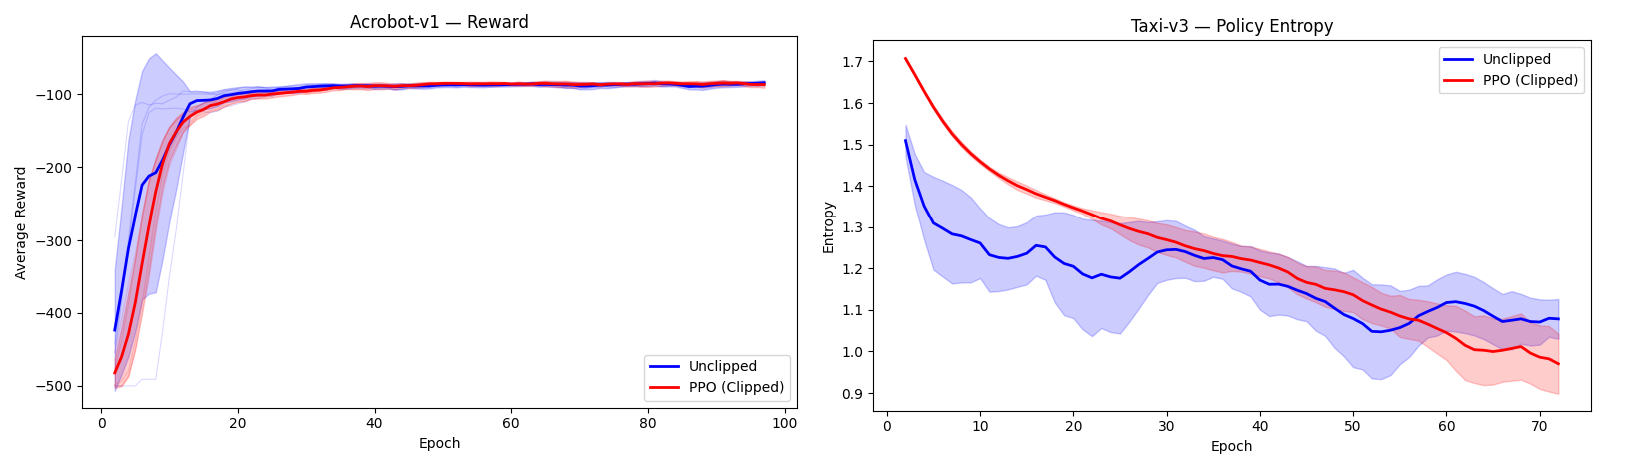
\includegraphics[width=\linewidth]{figures/curves.png}
\end{center}
\caption{Left: CartPole-v1 reward curves for clipped and unclipped conditions across 4 seeds. Faint lines show individual seeds; bold lines show smoothed mean; shaded bands show $\pm1$ std. Right: Taxi-v3 policy entropy curves for both conditions. The unclipped policy's entropy collapses early, while PPO maintains exploration.}
\label{fig:curves}
\end{figure}

\section{Analysis}
\label{sec:analysis}

\subsection{Relationship to the Original Paper}

Our results support the central claim of \citep{schulman2017ppo}: that clipping the surrogate objective improves training stability when multiple epochs are performed on the same rollout. \citet{schulman2017ppo} demonstrate this on continuous MuJoCo control tasks, reporting a normalized score of $-0.39$ (unclipped) vs $0.82$ (clipped) at $\varepsilon=0.2$ (Table~1). While our evaluation uses discrete-action environments rather than continuous control, the directional finding is consistent: the unclipped objective produces less stable learning dynamics across multiple environments.

The most direct correlation with the findings of the original paper is found in CartPole-v1. The unclipped baseline's high cross-seed variance ($\pm 147.01$) and late-training instability (std 138.97) reflect the destructive update behavior that \citet{schulman2017ppo} describe:

\begin{quote}
``performing multiple steps of optimization on this loss using the same trajectory\ldots empirically\ldots often leads to destructively large policy updates.''
\end{quote}

PPO's zero cross-seed variance and four-fold reduction in late-training standard deviation on the same environment provide small-scale empirical confirmation of this claim.

\subsection{The Two Failure Modes of the Unclipped Objective}

Our results reveal two distinct failure modes of the unclipped surrogate across environments:

\textbf{Instability.} In CartPole-v1, the unclipped objective produces high variance across seeds, with individual runs diverging significantly during late training. This is the failure mode \citet{schulman2017ppo} primarily describe, where unconstrained probability ratios allow updates that overshoot, destabilizing previously learned behavior.

\textbf{Premature collapse.} In Taxi-v3, the unclipped objective produces the opposite symptom: extremely low variance but locked into a suboptimal policy. The entropy collapse visible in Figure~\ref{fig:curves} confirms the policy has become near-deterministic early in training. This is a subtler manifestation of the same underlying problem: without clipping, large updates over multiple epochs can drive the policy toward overconfident, low-entropy behavior before sufficient exploration has occurred. Clipping prevents this by limiting how aggressively the policy can be updated in any single epoch.

Both failure modes, divergence and premature collapse, are symptoms of the same underlying instability, and both are mitigated by clipping, as shown in this project.

\subsection{Limitations}

Several limitations may have affected the scope of our conclusions:

\textbf{Training duration.} The limited number of epochs used in our testing explain the lack of meaningful results on LunarLander-v3, which reflect mid-training behavior rather than final performance.

\textbf{Discrete vs.\ continuous environments.} \citet{schulman2017ppo} evaluated their training primarily on continuous MuJoCo tasks whereas our evaluation uses discrete-action environments, which differ in reward structure, state space complexity, and the nature of policy collapse. While the directional findings are consistent, the magnitude of the effect may differ from the original paper's results.

\textbf{Seed count.} Four seeds per condition is sufficient to observe trends but limits the statistical reliability of the results. A larger seed count could potentially produce more robust estimates of variance.

\textbf{Hyperparameter sensitivity.} Our hyperparameters are held fixed across all environments. Environment-specific tuning would likely improve the performance for both conditions, but was deliberately avoided to ensure clipping remains the sole independent variable.


\section{Conclusion}

In this project, we present a small-scale reproduction of the stability claim made by \citep{schulman2017ppo}: that PPO's clipped surrogate objective ($L^{CLIP}$) produces more stable training than the unclipped importance-sampled surrogate ($L^{CPI}$) when multiple epochs are performed on the same rollout. Our experiments isolate clipping as the sole independent variable and hold all other components fixed between conditions.

The results found in four discrete-action environments provide consistent support for this claim. On CartPole-v1, the clipped objective achieves maximum reward with zero cross-seed variance, while the unclipped baseline exhibits high variance and late-training instability. On Taxi-v3, the unclipped objective undergoes premature entropy collapse and insufficient exploration, which is a subtler but equally damaging form of instability. These two environments reveal distinct failure modes of the unclipped objective: divergence and premature convergence, both diminished by clipping.

Results on Acrobot-v1 and LunarLander-v3 are inconclusive, reflecting limitations in training duration rather than the method itself, verifying that clipping works best in stress-based environments. Future work should extend training to more epochs and evaluate on continuous-action environments to more directly replicate the conditions of the original paper.

Our implementation reproduces the same architecture and training procedure of \citep{schulman2017ppo}, using the same two-layer 64-unit MLP with tanh activations and the same core hyperparameters. At a small scale and in discrete environments, our results are consistent with the original finding that clipping the probability ratio provides a simple and effective mechanism for stabilizing policy gradient training under multiple optimization epochs.

\section*{LLM Acknowledgments}
Claude (Anthropic) was used during the preparation of this manuscript for the following purposes: reviewing the paper to help adhere to guidelines set by ICLR 2026 conference. 

ChatGPT was used during the preparation of this manuscript for the following purposes: (1) suggesting structural edits such as condensing the introduction; (2) editing prose for better grammar structure; (3) fixing citations.

No LLM was used to generate code.


\bibliography{refs}
\bibliographystyle{iclr2026_conference}

\end{document}
